\chapter{Apparent Regime Shifts or Nonlinear State-Dependence?}
\label{chap_salmon_regimes}

\section{Abstract}
Natural systems that exhibit complex, nonlinear dynamics can undergo sudden changes characterized as regime shifts. A prominent example is the correlation between the Pacific Decadal Oscillation (PDO) and Pacific salmon, where salmon productivity is notably higher or lower depending on whether the PDO regime is warm or cold. Indeed, studies have found that salmon recruitment is better explained by separate stock-recruitment relationships for each PDO regime. However, this apparent relationship may actually represent a mirage correlation, a phenomenon known to occur when variables interact in a nonlinear system. Using nonparametric Empirical Dynamic Modeling (EDM), we fit  multivariate models to time series data of Fraser River sockeye salmon recruitment. We find no significant differences in forecasts when partitioning the data into different possible regimes, and thus no evidence supporting regime-specific recruitment dynamics. Rather, the observed correlation between the PDO and Pacific salmon productivity is likely a manifestation of nonlinear dynamics that gives the appearance of regime shifts even though the underlying system is unchanged.

\section{Introduction}

A central question in fisheries science, dating back at least a century to Hjort's seminal work \cite{Hjort_1914} is to understand the factors that influence recruitment. To date, various hypotheses have been proposed: tn the case of Pacific salmon populations, early work by Ricker on fitting stock-recruitment relationships suggested density-dependence as a mechanism \cite{Ricker_1954}. Another prominent hypothesis has been the influence of environmental variability on recruitment \cite{Cushing_1982}. Here, an early study by \cite{Ricker_1958}, again on Pacific salmon, found no evidence for environmental effects. However, this negative result may be caused by the limited statistical power of the data available at the time (Richard Beamish, personal communication, May 27, 2014).

More recent work has identified correlations between decadal scale climate indices (e.g., Pacific Decadal Oscillation, PDO; Aleutian Low Pressure Index, ALPI) and Pacific salmon productivity \cite{Mantua_1997, Beamish_1997}. These results suggest that there is indeed some form of physical-biological coupling between salmon populations and the environment. Indeed, when the data are partitioned by climate regime, standard stock-recruitment curves actually fit better for pink and sockeye salmon from the Fraser River \cite{Beamish_2004a}, suggesting that there are trends in survival and productivity related to climate.

One of the implications of regime-dependent behavior or parameters is that models will perform better when fit to data from exactly one regime (\`{a} la \cite{Beamish_2004a}). When the system transitions into a new regime, models based on data from a different regime may no longer be predictive. A correct understanding of the causes for observed shifts in populations is thus critical for fisheries management, to distinguish between natural impacts caused by biological or physical mechanisms, and fishing effects that could potentially be controlled through regulation and management \cite{Beamish_1999}. A failure to consider the possibility of changing system dynamics can lead to misguided or ineffective management, such as in the case of prolonged recovery of Northwest Atlantic cod \cite{Shelton_2011a}.

Although regime shifts appear quite common in marine fish stocks \cite{Vert-pre_2013}, the hallmark features of regime shifts are also characteristic of nonlinear systems. For example, time series from nonlinear systems often exhibit red noise power spectra, which can be erroneously identified as regime shifts \cite{Rudnick_2003}. Moreover, the defining feature of nonlinear systems is that variable interactions are state-dependent and change as a function of system state. Slow changes in the these interactions over time could be interpreted as regime shifts when linear models are applied, just as simple nonlinear functions can be approximated by piece-wise linear segments. Finally, a prime example of nonlinear phenomena that can give the appearance of changing dynamics is that of ``mirage correlations'', transient artifacts that can appear in coupled dynamic systems \cite{Sugihara_2012}. There is growing evidence that mirage correlations are prevalent in marine fisheries, with many studies showing inconsistent correlations as longer time series are collected \cite{Myers_1998, McClatchie_2010, Litzow_2014a}. Thus, the apparent regime-like behavior of Pacific salmon populations may not reflect changing behavior, but could actually be indicative of nonlinearity.

Here, we utilize the approach of empirical dynamic modeling (EDM) to examine the possibility of regime-dependent dynamics in Fraser River sockeye salmon. We consider four hypotheses for the number of distinct ``regimes'' over the time span of our data:
\begin{itemize}
\item[I] Four different time periods \cite{Beamish_2004a}: 1948-1976, 1977-1988, 1989-1998, and 1999-present
\item[II] Three different time periods \cite{Litzow_2014}: 1948-1976, 1977-1998, 1999-present
\item[III] Two different time periods \cite{McGowan_2003}: 1948-1976, 1977-present
\item[IV] One time period (null hypothesis): 1948-present
\end{itemize}

For each hypothesis, we fit multivariate EDM models \cite{Dixon_1999} to data from each time period separately, producing up to four different models. This procedure is then repeated for each of the nine most historically abundant stocks of sockeye salmon in the Fraser River: Birkenhead, Chilko, Early Stuart, Late Stuart, Late Shuswap, Quesnel, Seymour, Stellako, and Weaver. As shown in previous work \cite{Ye_2015}, EDM methods can accommodate nonlinearity as well as state-dependent environmental effects. Thus, this approach is ideally suited to distinguish between actual shifts in dynamics across hypothesized regimes and the illusion of change when linear models are applied to nonlinear systems.

\section{Results}

\begin{figure}[!ht]
\begin{center}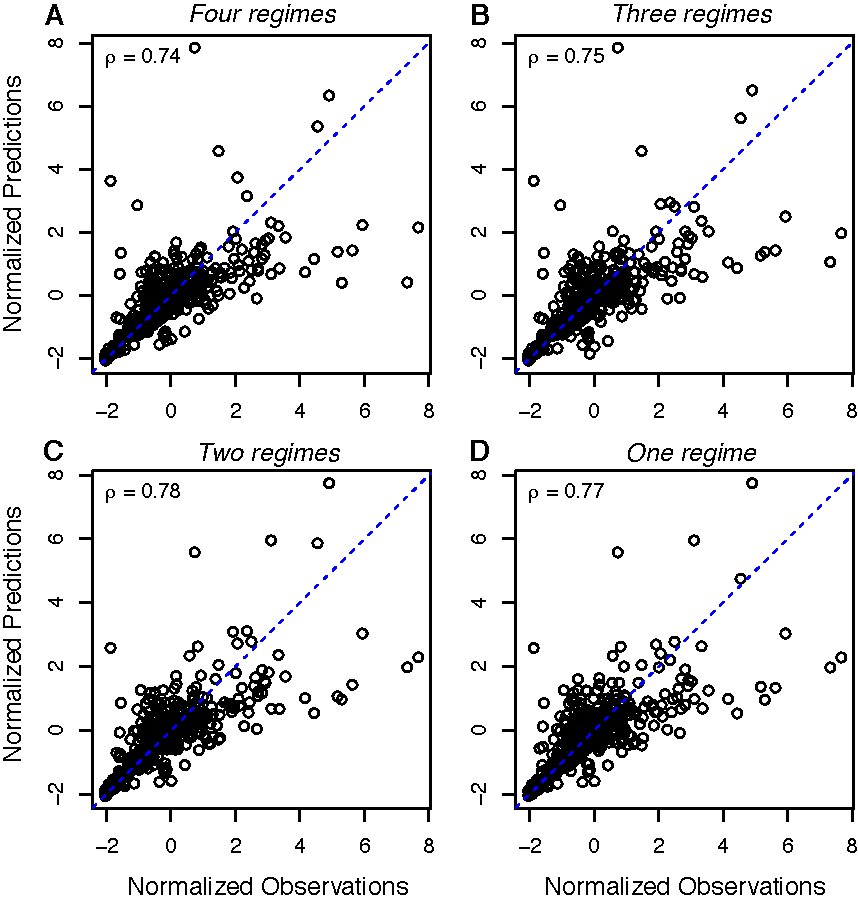
\includegraphics[width=\maxwidth{\textwidth}]{fig_regimes_1.pdf}\end{center}
\caption[Aggregated forecast accuracy for different regime hypotheses.]{\textbf{Aggregated forecast accuracy for different regime hypotheses.}\newline
(A) Normalized predictions vs. normalized observations, aggregated over the nine historically most abundant stocks. For each stock, models are fit separately to the four time periods of hypothesis I. (B-D) Same as (A), but for hypotheses II, III, and IV, respectively. Forecast skill is nearly identical across the four hypotheses, indicating no evidence for regime-specific behavior.}
\label{fig_regimes_aggregated_forecast_skill}
\end{figure}

Figure \ref{fig_regimes_aggregated_forecast_skill} shows predictions vs. observed values for the four different hypotheses and aggregated over the nine stocks examined here. Note that because the stocks have different mean population sizes, the forecasts and actual values for each stock are normalized to mean = 0, and variance = 1. It is visually apparent that there are very few differences in forecast skill across the four hypotheses, and confirmed by the computed forecast accuracy numbers ($\rho$, correlation coefficient between predicted and observed, in the upper left corner of each panel).

\begin{table}[!ht]
\caption[Stock-specific forecast skill for different regime hypotheses.]{\textbf{Stock-specific forecast skill for different regime hypotheses.}\newline
$\rho$, correlation coefficient between observations and predictions; MAE, mean absolute error.}
\label{tab_regimes_full_forecast_skill}
\begin{center}
\resizebox{\textwidth}{!}{
% latex table generated in R 3.2.0 by xtable 1.7-4 package
% Mon Aug 24 12:39:42 2015
\begin{tabular}{llrrrr}
  \hline
stock & metric & Four regimes & Three regimes & Two regimes & One regime \\ 
  \hline
Early Stuart & $\rho$ & 0.893 & 0.896 & 0.884 & 0.882 \\ 
  & MAE & 0.124 & 0.118 & 0.130 & 0.124 \\ 
  Seymour & $\rho$ & 0.781 & 0.777 & 0.775 & 0.762 \\ 
  & MAE & 0.056 & 0.057 & 0.056 & 0.058 \\ 
  Chilko & $\rho$ & 0.396 & 0.360 & 0.418 & 0.393 \\ 
  & MAE & 0.778 & 0.781 & 0.750 & 0.751 \\ 
  Late Stuart & $\rho$ & 0.760 & 0.750 & 0.794 & 0.791 \\ 
  & MAE & 0.316 & 0.316 & 0.296 & 0.304 \\ 
  Quesnel & $\rho$ & 0.554 & 0.603 & 0.706 & 0.705 \\ 
  & MAE & 1.068 & 1.029 & 0.916 & 0.925 \\ 
  Stellako & $\rho$ & 0.607 & 0.536 & 0.505 & 0.446 \\ 
  & MAE & 0.206 & 0.215 & 0.222 & 0.241 \\ 
  Birkenhead & $\rho$ & 0.572 & 0.615 & 0.538 & 0.481 \\ 
  & MAE & 0.180 & 0.171 & 0.189 & 0.213 \\ 
  Late Shuswap & $\rho$ & 0.873 & 0.886 & 0.872 & 0.867 \\ 
  & MAE & 0.840 & 0.809 & 0.887 & 0.880 \\ 
  Weaver & $\rho$ & 0.812 & 0.791 & 0.743 & 0.729 \\ 
  & MAE & 0.130 & 0.136 & 0.149 & 0.158 \\ 
   \hline
\end{tabular}

}
\end{center}
\end{table}

Table \ref{tab_regimes_full_forecast_skill} lists the forecast accuracy ($\rho$,  correlation coefficient between observations and predictions) and forecast error (MAE, mean absolute error) for each individual stock under the four different hypotheses. In general, there are no large differences in forecast skill across the four hypotheses. For some stocks (e.g., Quesnel, Birkenhead, Weaver), forecast skill is more variable across the different hypotheses; however, no pairwise comparisons are significant at the $p = 0.05$ level for either forecast accuracy ($\rho$) or forecast error (MAE) (see Methods for details of statistical tests).

\section{Discussion}

Our results (Figure \ref{fig_regimes_aggregated_forecast_skill} and Table \ref{tab_regimes_full_forecast_skill}) show no evidence that Fraser River sockeye salmon have regime-specific dynamics. This may not be surprising given that earlier studies in this system reported nonlinear dynamics and state-dependent environmental interactions \cite{Ye_2015}. However, even so, we might have expected forecasts to be better when different models could be fit separately to the different time periods. By selecting the best model for each time period, and using leave-one-out cross-validation to produce forecasts (see Methods), any differences in dynamics across regimes should appear as improvements in forecast skill. Given that performance was virtually identical across the four hypotheses, we conclude that there is no benefit to partitioning the data by climate regimes when modeling recruitment. Nevertheless, we consider several alternative explanations for our results.

\subsection{Alternative Explanations}

One possibility is that the nearest-neighbor forecasting method used in our EDM models is flexible enough to account for regime-specific dynamics, thus yielding equivalent performance for the``one-regime'' and ``multi-regime'' hypotheses. Because simplex projection makes predictions based on nearest neighbors (i.e., the historical times best judged to be similar states of the system) it could be the case that points from different regimes are simply accurately identified as \emph{not} being nearest neighbors. For example, the system behavior for the 1950-1976 time period could be quite different from that of the 1977-present time period, and when EDM is applied, the data from these two time periods are localized to different regions of the reconstructed state space. Thus, points in a different regime would not be selected as nearest neighbors, and forecast performance would be equivalent to fitting separate models to the different regimes. Even so, we might expect better forecasts when partitioning the data into regimes, because the model for each time period can be different. In other words, the most predictive set of environmental variables might be different across regimes, thereby yielding better forecast skill for the ``multi-regime'' hypothesis. However, this does not appear to occur, suggesting that there are no performance advantages to allowing the model to change over time.
%By selecting the best model for each time period, forecasts can improve in the ``multi-regime'' framework if the most predictive set of environmental variables changes.
%That this does not occur, suggests that in at least some cases, there are nearest neighbors selected from different time periods, thus providing an effective data advantage when fitting a single model to the entire time series.

Another possible explanation is that the variables used in this study are not informative enough to differentiate between regime-specific dynamics. As noted in \cite{Ye_2015}, these environmental variables are hypothesized to be proxies for juvenile food availability. Thus, while the relationship between recruitment dynamics and the tested environmental variables does not appear to be regime-specific, this may reflect the incompleteness of using an environmental measure as a proxy. In other words, it may be the case that the relationship between food availability and recruitment \emph{is} regime-specific, but that the mapping between food availability and the environmental proxies is not. As such, information is lost when using the environment as an imperfect proxy; this would explain both the imperfect forecast skill and the lack of improvement in forecasts when partitioning the data into different time periods. This data limitation could be overcome by including more direct measurements of the system. For instance trawl surveys of the Strait of Georgia should be more informative about actual food availability \cite{Beamish_2000}. Although these data do not extend far back enough to re-examine the regime shift question, it would still be possible to determine whether they are more relevant for predicting recruitment compared to indirect environmental proxies.

\subsection{Nonlinearity}

Like other studies \cite{Hsieh_2005, Glaser_2014}, our results contribute to growing evidence of nonlinear dynamics in marine fish stocks. An important distinction between the nonlinear perspective and that of the regime shift perspective relates to how data are used to construct models. In both frameworks, future behavior can be estimated by examining similar historical states. However, whereas the EDM approach identifies similar states based on location within the reconstructed state space, a regime shift perspective would identify similar states based on their proximity in time (i.e., points belonging to the same regime). In cases where the the system occupies similar regions of the state-space (perhaps due to red-noise spectra of important environmental factors), the resulting dynamics may thus appear to be time-dependent. In other words, the appearance of regime shifts can result from the nonlinear interaction of biological populations with red-noise-like environmental forcing.

We also note that aggregating data across multiple nonlinear systems is known to obscure nonlinear signals \cite{Sugihara_1994}. As such, the prominent correlations of Pacific salmon productivity with North Pacific climate \cite{Mantua_1997, Beamish_1997} may be a simplification of the true system behavior and the result of averaging over state-dependent interactions at the individual stock level. While such a coarse description of environmental impacts may be useful for predicting regional long-term trends (e.g., due to climate change), it ignores important nonlinear interactions that are potentially important for fisheries management on smaller spatial scales.

\section{Conclusions}

We find no evidence that Fraser River sockeye salmon dynamics change across different regimes of North Pacific Ocean climate. Rather, our results suggest that the apparent changes in mean salmon abundance reflect nonlinear interactions between stochastic environment and salmon biology. Moreover, because aggregating multiple nonlinear signals can result in linearity \cite{Sugihara_1994}, the observed correlations between salmon productivity and climate indices \cite{Mantua_1997, Beamish_1997} are likely the result of combining time series from multiple stocks into a single measure of \emph{regional} salmon productivity, and inadvertently diminishing the nonlinear signal.

The distinction between nonlinearity and regime-shift dynamics has important implications for fisheries management. If populations are influenced by the interaction of multiple factors (including fishing, the environment, and species interactions), correct accounting of these influences is necessary for effective management. As shown here, nonlinear, equation-free approach of EDM can accomplish the task of forecasting recruitment where traditional mathematical models would suggest that system behavior is tied to climate regimes. Nevertheless, the regime shift framework may be useful in some cases, for instance, when data are not available to identify nonlinear interactions. However, with sufficient observations, established patterns may eventually break down \cite{Litzow_2014a}, necessitating a more realistic and nonlinear worldview.

\section{Methods}

\subsection{Data}

Following \cite{Ye_2015}, we analyze yearly time series data for the 9 historically most abundant stocks (Birkenhead, Chilko, Early Stuart, Late Shuswap, Late Stuart, Quesnel, Seymour, Stellako, and Weaver) of sockeye salmon from the Fraser River system. Data span brood years 1948--2005, except for Late Stuart and Weaver, where data begin in 1949 and 1966, respectively.

Population data consists of two biological variables: stock size (number of effective female spawners) and recruitment (returning adults. Recruitment is also partitioned by age; following \cite{Grant_2010}, we consider only age 4 and age 5 recruits.

Environmental data consists of three variables: the Pacific Decadal Oscillation (PDO), sea-surface temperature (SST), and Fraser River discharge. As in \cite{Ye_2015}, one annual time series is constructed for the PDO as the average of monthly values from November to March \cite{Mantua_1997}, SST measures are monthly averages from two lighthouse stations (Entrance Island: April to June and Pine Island: April to July), and river discharge is measured at Hope (including both peak daily flow for the year, and monthly averages from April to June).

Because the identified regimes pertain to the physical conditions of the North Pacific, and the environmental data are believed to influence sockeye salmon recruitment at age 2, we partition the data according based on when the corresponding environmental measures fall in one regime or another. That is, if 1948-1976 is one physical regime, the relevant biological data for that regime corresponds to brood years 1946-1974, with age 4 recruits appearing in calendar years 1950-1978.

Data are partitioned in one, two, three, or four different time periods according to descriptions of North Pacific regimes in \cite{McGowan_2003, Beamish_2004a, Litzow_2014}:
\begin{itemize}
\item[I] Four different time periods: 1948-1976, 1977-1988, 1989-1998, and 1999-present
\item[II] Three different time periods: 1948-1976, 1977-1998, 1999-present
\item[III] Two different time periods: 1948-1976, 1977-present
\item[IV] One time period: 1948-present
\end{itemize}
As noted above, these years refer to calendar years for the physical environment. The corresponding brood years are shifted 2 years earlier.

\subsection{Model Construction and Performance}

Following \cite{Ye_2015}, we use multivariate simplex projection. For each combination of stock and time period, we examine models that include spawning stock size and up to 2 environmental variables. Forecasts for each model were produced using leave-one-out validation: for each forecast, the model was fit to data that excluded the corresponding stock size and environmental data. Although \cite{Ye_2015} used four-fold cross-validation to estimate out-of-sample forecast performance, several of the time periods examined here are much shorter and not suitable for such subdivision of the data.

Forecasts were produced for both age 4 and age 5 recruits before summing to obtain total recruitment for each brood year. (Note that this recruitment happens over two consecutive calendar years, with age 4 recruits appearing 4 years after spawning, and age 5 recruits appearing 5 years after spawning.) For each combination of stock and time period, the model producing the highest model accuracy ($\rho$, described below) was selected.

Model performance is quantified using Pearson's correlation coefficient ($\rho$) between observed and predicted returns as a measure of accuracy and MAE (mean absolute error) as a measure of error. Comparisons of $\rho$ between models uses a one-sided $t$ test with SE calculated using the HC4 estimator from \cite{Cribari-Neto_2004} and with adjusted degrees of freedom as suggested by \cite{Wilcox_2009}. Differences in MAE were computed using a paired $t$ test for the difference, treating each forecast as an independent sample.

To compute an aggregate statistic combining all 9 stocks, we first scale the observations and predictions for each stock so that the observed returns have mean $= 0$, variance $= 1$, and then combine the normalized values across stocks (Figure \ref{fig_regimes_aggregated_forecast_skill}).

\section{Acknowledgments}
This research is supported by Department of Defense, Strategic Environment Research and Development Program RC-2509 (GS, HY), Lenfest Ocean Program \#00028335 (GS), National Science Foundation Grant No. DEB-1020372 (GS, HY), NSF-NOAA Comparative Analysis of Marine Ecosystem Organization (CAMEO) program Grant NA08OAR4320894/CAMEO (GS), National Science Foundation Graduate Research Fellowships (HY), the Sugihara Family Trust (GS), the Deutsche Bank-Jameson Complexity Studies Fund (GS), and the McQuown Chair in Natural Science (GS).

Chapter \ref{chap_salmon_regimes}, in full, is material prepared for submission: Hao Ye and George Sugihara. Apparent regime shifts or nonlinear state-dependence: Environmental drivers of Fraser River sockeye salmon recruiment. The dissertation author was the primary investigator and author of this paper.